\setcounter{chapter}{8}
\chapter{Forecasting and Time Series Models}
{\small \textit{Chapter Preview}.  This chapter introduces two
popular smoothing techniques, moving (running) averages and
exponential smoothing, for forecasting. These techniques are simple
to explain and easily interpretable. They can be also expressed as
regression models, where the technique of weighted least squares is
used to compute parameter estimates. Seasonality is then presented,
followed by a discussion of two more advanced time series topics,
unit root testing and volatility (\textit{ARCH/GARCH}) models.}


\section{Smoothing with Moving Averages}


Smoothing a time series with a moving, or running, average, is a
time tested procedure. This technique continues to be used by many
data analysts because of its ease of computation and resulting ease
of interpretation. As we discuss below, this estimator can also be
motivated as a weighted least squares (WLS) estimator. Thus, the
estimator enjoys certain theoretical properties.

The basic \emph{moving, or running, average estimate} is defined by
\begin{equation}\label{E9:MovingAverage1}
\widehat{s}_t = \frac{y_t + y_{t-1} + \ldots + y_{t-k+1}}{k} ,
\end{equation}
where $k$ is the \emph{running average length}. The choice of $k$
depends on the amount of smoothing desired. The larger the value of
$k$, the smoother is the estimate $\widehat{s}_t$ because more
averaging is done. The choice $k=1$ corresponds to no
smoothing.\index{time series statistics!moving average
estimate}\index{time series statistics!running average estimate}

\empexjed{MedCPISmooth}

\subsubsection*{Application: Medical Component of the CPI}\ecaptionjed{Medical Component of the CPI}
\index{datasets!medical price inflation}

The consumer price index (CPI) is a breadbasket of goods and
services whose price is measured in the US by the Bureau of Labor
Statistics. By measuring this breadbasket periodically, consumers
get an idea of the steady increase in prices over time which, among
other things, serves as a proxy for inflation. The CPI is composed
of many components, reflecting the relative importance of each
component to the overall economy. Here, we study the medical
component of the CPI, the fastest growing part of the overall
breadbasket since 1967. The data we consider are quarterly values of
the medical component of the CPI (MCPI) over a sixty year period
from 1947 to the first quarter of 2007, inclusive. Over this period,
the index rose from 13.3 to 346.0. This represents a twenty-six fold
increase over the sixty year period which translates into a 1.36\%
quarterly increase.

Figure \ref{F9:MCPISmooth} is a time series plot of quarterly
percentage changes in MCPI. Note that we have already switched from
the nonstationary index to percentage changes. (The index is
nonstationary because it exhibits such a tremendous growth over the
period considered.) To illustrate the effect of the choice of $k$,
consider the two panels of Figure \ref{F9:MCPISmooth}. In the upper
panel of Figure \ref{F9:MCPISmooth}, the smoothed series with $k=4$
is superimposed on the actual series. The lower panel is the
corresponding graph with $k=8$. The fitted values in the lower panel
are less jagged than those in upper panel. This helps us to identify
graphically the real trends in the series. The danger in choosing
too large a value of $k$ is that we may ``over-smooth'' the data and
lose sight of the real trends.


\begin{figure}[htp]
  \begin{center}
    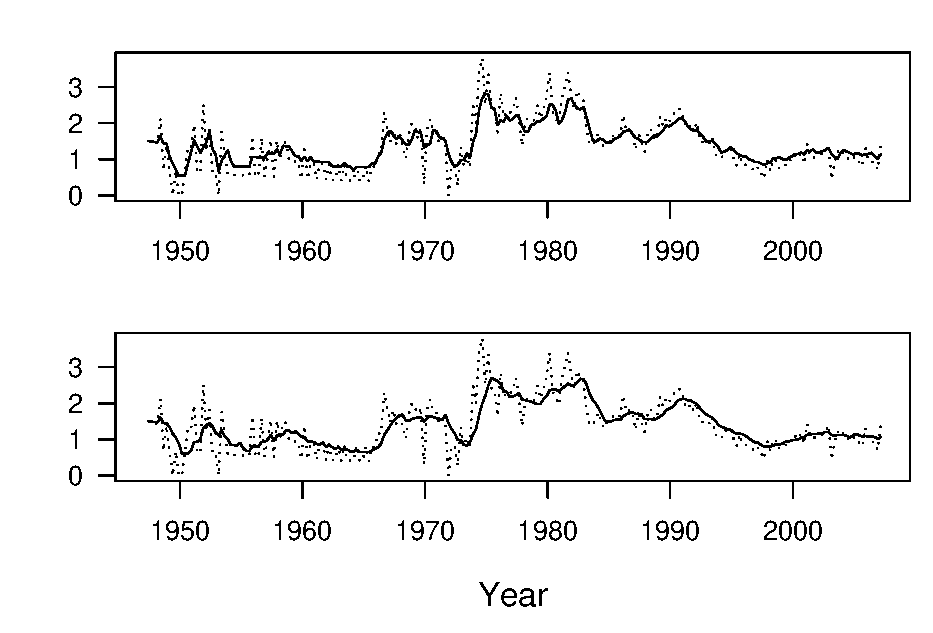
\includegraphics[width=1\textwidth]
     {Chapter9Forecasting/MCPISmooth.eps}
    \caption{\label{F9:MCPISmooth} \small Quarterly
Percentage Changes in the Medical Component of the Consumer Price
Index. For both panels , the dashed line is the index. For the upper
panel, the solid line is the smoothed version with $k$=4. For the
lower panel, the solid line is the smoothed version with $k$=8.
\emph{Source}: Bureau of Labor Statistics}
  \end{center}
\end{figure}


\bigskip
To forecast the series, re-express equation
(\ref{E9:MovingAverage1}) recursively to get
\begin{equation}\label{E9:MovingAverag2}
\widehat{s}_t = \frac{y_t + y_{t-1} + \ldots + y_{t-k+1}}{k} =
\frac{y_t + k \widehat{s}_{t-1} - y_{t-k}}{k} = \widehat{s}_{t-1} +
\frac{y_t-y_{t-k}}{k}.
\end{equation}
If there are no trends in the data, then the second term on the
right hand side, $(y_t-y_{t-k})/k$, may be ignored in practice. This
yields the forecasting equation $\widehat{y}_{T+l} = \widehat{s}_T$
for forecasts $l$ lead time units into the future.

Several variants of running averages are available in the
literature. For example, suppose that a series can be expressed as
$y_t = \beta_0 + \beta_1 t + \varepsilon_t$, a linear trend in time
model. This can be handled through the following \emph{double
smoothing} procedure:\index{time series terms and concepts!double
smoothing}

\begin{enumerate}
\item Create a smoothed series using equation (\ref{E9:MovingAverage1}), that
is, $\widehat{s}_t^{(1)}=(y_t+\ldots+y_{t-k+1})/k.$

\item Create a doubly smoothed series by using equation (\ref{E9:MovingAverage1})
and treating the smoothed series created in step (i) as input. That
is, $\widehat{s}_t^{(2)} = (\widehat{s}_t^{(1)} + \ldots +
\widehat{s}_{t-k+1}^{(1)})/k.$
\end{enumerate}
It is easy to check that this procedure smooths out the effect of a
linear trend in time. The estimate of the trend is $b_{1,T}=2\left(
\widehat{s}_T^{(1)}-\widehat{s}_T^{(2)}\right) /(k-1)$. The
resulting forecasts are $\widehat{y}_{T+l} = \widehat{s}_T +
b_{1,T}~l$ for forecasts $l$ lead time units into the future.

\subsubsection*{Weighted Least Squares}

An important feature of moving, or running, averages is that they
can be expressed as weighted least squares (WLS) estimates. WLS
estimation was introduced in Section 5.7.3. You will find additional
broad discussion in Section 15.1.1. Recall that WLS estimates are
minimizers of a weighted sum of squares. The WLS procedure is to
find the values of $b_0^{\ast}, \ldots, b_{k}^{\ast}$ that
minimize

\marginparjed{WLS estimation was introduced in Section 5.7.3 and is
further described in Section 15.1.1.}

\begin{equation}\label{E9:WSS}
WSS_T\left( b_0^{\ast },\ldots, b_k^{\ast}\right) = \sum_{t=1}^{T}
w_t \left( y_t-\left( b_0^{\ast} + b_1^{\ast} x_{t1}, \ldots,
b_{k}^{\ast} x_{tk} \right) \right)^2.
\end{equation}
Here, $WSS_T$ is the weighted sum of squares at time $T$.

To arrive at the moving, or running, average estimate, we use the
model $ y_t = \beta_0 + \varepsilon_t$ with the choice of weights
$w_t=1$ for $t = T-k+1, \ldots, T$ and $w_t=0$ for $t<T-k+1$. Thus,
the problem of minimizing $WSS_T$ in equation (\ref{E9:WSS}) reduces
to finding $b_0^{\ast}$ that minimizes $\sum_{t=T-k+1}^{T}\left( y_t
- b_0^{\ast} \right)^2.$ The value of $b_0^{\ast}$ that this
expression is $b_0 = \widehat{s}_T$, which is the running average of
length $k$.

This model, together with this choice of weights, is called a
\emph{locally constant mean model}. Under a \emph{globally constant
mean model}, equal weights are used and the least squares estimate
of $\beta_0$ is the overall average, $\overline{y}$. Under the
locally constant mean model, we give equal weight to observations
within $k$ time units of the evaluation time $T$ and zero weight to
other observations. Although it is intuitively appealing to give
more weight to more recent observations, the notion of an abrupt
cut-off at a somewhat arbitrarily chosen $k$ is not appealing. This
criticism is addressed using exponential smoothing, introduced in
the following section.

\section{Exponential Smoothing}\label{S9:ExponSmooth}

Exponential smoothing estimates are weighted averages of past values
of a series, where the weights are given by a series that becomes
exponentially small. To illustrate, think of $w$ as a weight number
that is between zero and one and consider the weighted average
\begin{equation*}
\frac{y_t + w y_{t-1} + w^2 y_{t-2} + w^3 y_{t-3} +
\ldots}{1/(1-w)}.
\end{equation*}
This is a weighted average because the weights $w^k (1-w)$ sum to
one, that is, a geometric series expansion yields
$\sum_{k=0}^{\infty }w^k = 1/(1-w)$.

Because observations are not available in the infinite past, we use
the truncated version
\begin{equation}\label{E9:ExponSmooth1}
\widehat{s}_t = \frac{y_t + w y_{t-1} + \ldots + w^{t-1} y_1 +
\ldots + w^t y_0}{1/(1-w) }
\end{equation}
to define the \emph{exponential smoothed estimate} of the series.
Here, $y_0$ is the starting value of the series and is often chosen
to be either zero, $y_1$, or the average value of the series,
$\overline{y}$. Like running average estimates, the smoothed
estimates in equation (\ref{E9:ExponSmooth1}) provide greater
weights to more recent observations as compared to observations far
in the past with respect to time $t$. Unlike running averages, the
weight function is smooth.\index{time series statistics!exponential
smoothed estimate}

The definition of exponential smoothing estimates in equation
(\ref{E9:ExponSmooth1}) appears complex. However, as with running
averages in equation (\ref{E9:MovingAverag2}), we can re-express
equation (\ref{E9:ExponSmooth1}) recursively to yield
\begin{equation}\label{E9:ExponSmooth2}
\widehat{s}_t = \widehat{s}_{t-1} + (1-w)(y_t-\widehat{s}_{t-1}) =
(1-w) y_t + w \widehat{s}_{t-1}.
\end{equation}
The expression of the smoothed estimates in equation
(\ref{E9:ExponSmooth2}) is easier to compute than the definition in
equation (\ref{E9:ExponSmooth1}).

Equation (\ref{E9:ExponSmooth2}) also provides insights into the
role of $w$ as the smoothing parameter. For example, on one hand as
$w$ gets close to zero, $\widehat{s}_t$ gets close to $y_t$. This
indicates that little smoothing has taken place. On the other hand,
as $w$ gets close to one, there is little effect of $y_t$ on
$\widehat{s}_t$. This indicates that a substantial amount of
smoothing has taken place because the current fitted value is almost
entirely composed of past observations.

\linejed

\textbf{Example: Medical Component of the CPI - Continued.} To
illustrate the effect of the choice of the smoothing parameter,
consider the two panels of Figure \ref{F9:MCPIESmooth}. These are
time series plots of the quarterly index of the medical component of
the CPI. In the upper panel, the smoothed series with $ w=0.2$ is
superimposed on the actual series. The lower panel is the
corresponding graph with $w=0.8$. From these figures, we can see
that the larger is $w$, the smoother are our fitted values.


\begin{figure}[htp]
  \begin{center}
    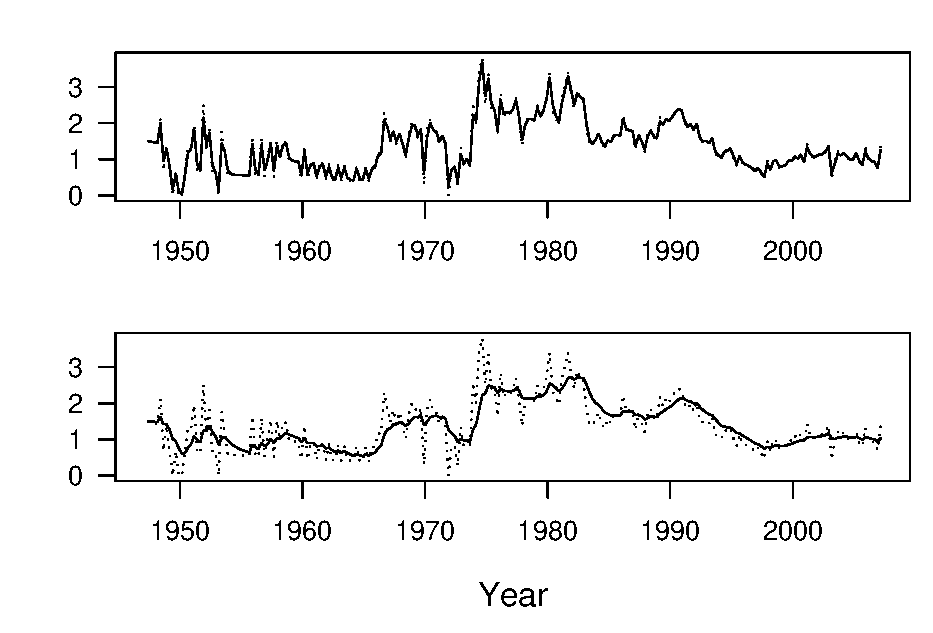
\includegraphics[width=1\textwidth]
     {Chapter9Forecasting/MCPIESmooth.eps}
    \caption{\label{F9:MCPIESmooth} \small Medical
Component of the Consumer Price Index with Smoothing. For both
panels, the dashed line is the index. For the upper panel, the solid
line is the smoothed version with $w$=0.2. For the lower panel, the
solid line is the smoothed version with $w$=0.8.}
  \end{center}
\end{figure}

\linejed

\bigskip

Equation (\ref{E9:ExponSmooth2}) also suggests using the relation
$\widehat{y}_{T+l} = \widehat{s}_T$ for our forecast of $y_{T+l}$,
that is, the series at $l$ lead units in the future. Forecasts not
only provide a way of predicting the future but also a way of
assessing the fit. At time $t-1$, our ``forecast'' of $y_t$ is
$\widehat{s}_{t-1}$. The difference is called the \emph{one-step
prediction error}.

To assess the degree of fit, we use the sum of squared one-step
prediction errors
\begin{equation}
SS\left( w\right) = \sum_{t=1}^T \left( y_t - \widehat{s}_{t-1}
\right)^2.
\end{equation}
An important thing to note is that this sum of squares is a function of the
smoothing parameter, $w$. This then provides a criterion for choosing the
smoothing parameter: choose the $w$ that minimizes $SS\left( w\right) $.
Traditionally, analysts have recommended that $w$ lie within the interval
(.70, .95), without providing an objective criterion for the choice.
Although minimizing $SS\left( w\right) $ does provide an objective
criterion, it is also computationally intensive. In absence of a
sophisticated numerical routine, this minimization is typically accomplished
by calculating $SS\left( w\right) $ at a number of choices of $w$ and
choosing the $w$ that provides the smallest value of $SS\left( w\right) $.

To illustrate the choice of the exponential smoothing parameter $w$,
we return to the medical CPI example. Figure \ref{F9:SSPE}
summarizes the calculation of $SS\left( w\right) $ for various
values of $w$. For this data set, it appears a choice of $w \approx
0.50$ minimizes $SS(w)$.


\begin{figure}[htp]
  \begin{center}
    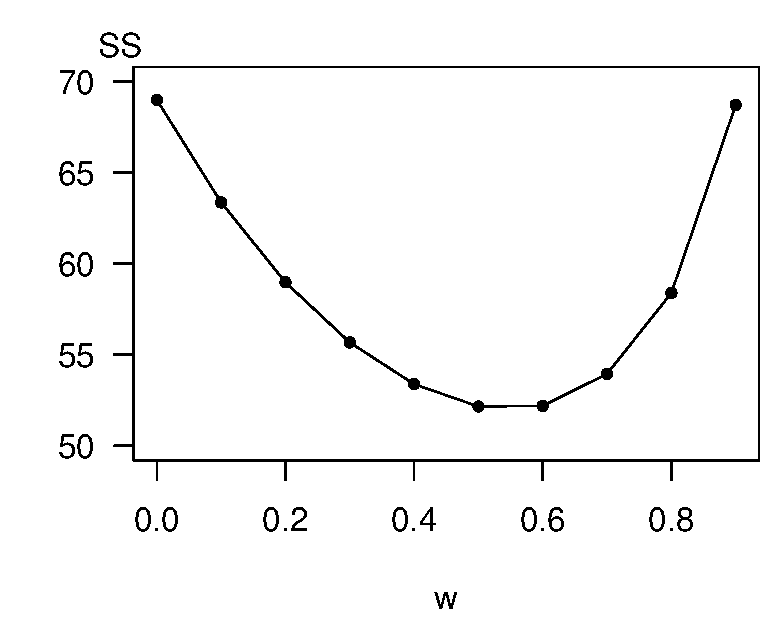
\includegraphics[width=.3\textwidth]
     {Chapter9Forecasting/SSPE.eps}
    \caption{\label{F9:SSPE} \small Sum of Squared One-Step Prediction Errors. Plot of the sum of squared prediction errors
$SS(w)$ as a function of the exponential smoothing parameter $w$.}
  \end{center}
\end{figure}


As with running averages, the presence of a linear trend in time,
$T_t = \beta_0 + \beta_1 t$, can be handled through the following
double smoothing procedure:

\begin{enumerate}
\item Create a smoothed series using equation (\ref{E9:ExponSmooth2}), that is,
$\widehat{s}_t^{(1)} = (1-w) y_t + w \widehat{s}_{t-1}^{(1)}.$

\item Create a doubly smoothed series by using equation (\ref{E9:ExponSmooth2})
and treating the smoothed series created in step (i) as input. That
is, $\widehat{s}_t^{(2)} = (1-w) \widehat{s}_t^{(1)} +
w\widehat{s}_{t-1}^{(2)}$.
\end{enumerate}

\noindent The estimate of the trend is $b_{1,T} =
((1-w)/w)(\widehat{s}_T^{(1)}- \widehat{s}_T^{(2)})$. The forecasts
are given by $\widehat{y}_{T+l}= b_{0,T}+b_{1,T}~l$ , where the
estimate of the intercept is $ b_{0,T} = 2\widehat{s}_T^{(1)} -
\widehat{s}_T^{(2)}$. We will also show how to use exponential
smoothing for data with seasonal patterns in Section
\ref{S9:SeasonalTSModels}.

\subsubsection*{Weighted Least Squares}

As with running averages, an important feature of exponentially
smoothed estimates is that they can be expressed as WLS estimates.
To see this, for the model $y_t = \beta_0 + \varepsilon_t,$ the
general weighted sum of squares in equation (\ref{E9:WSS}) reduces
to
\begin{equation*}
WSS_T\left( b_0^{\ast}\right) = \sum_{t=1}^T w_t \left( y_t -
b_0^{\ast} \right)^2.
\end{equation*}
The value of $b_0^{\ast}$ that minimizes $WSS_T\left( b_0^{\ast}
\right) $ is $b_0 = \left( \sum_{t=1}^T w_t y_t \right) / \left(
\sum_{t=1}^T w_t \right) $. With the choice $w_t = w^{T-t}$, we have
$b_0 \approx \widehat{s}_T$, where there is equality except for the
minor issue of the starting value. Thus, exponential smoothing
estimates are $WLS$ estimates. Further, because of the choice of the
form of the weights, exponential smoothing estimates are also called
\emph{discounted least squares estimates}. Here, $w_t=w^{T-t}$ is a
discounting function that one might use in considering the time
value of money.

\section{Seasonal Time Series Models}\label{S9:SeasonalTSModels}

Seasonal patterns appear in many time series that arise in the study
of business and economics. Models of seasonality are predominantly
used to address patterns that arise as the result of an
identifiable, physical phenomenon. For example, seasonal weather
patterns affect people's health and, in turn, the demand for
prescription drugs. These same seasonal models may be used to model
longer cyclical behavior.

There is a variety of techniques available for handling seasonal patterns
including fixed seasonal effects, seasonal autoregressive models, and
seasonal exponential smoothing methods. We address each of these techniques
below.

\subsubsection*{Fixed Seasonal Effects}\index{time series models!fixed seasonal effects}

Recall that, in equations (7.1) and (7.2), we used $S_t$ to
represent the seasonal effects under additive and multiplicative
decomposition models, respectively. A \emph{fixed seasonal effects
model} represents $S_t$ as a function of time $t$. The two most
important examples are the seasonal binary and trigonometric
functions. The Section 7.2 \textit{Trends in Voting Example} showed
how to use a seasonal binary variable and the \textit{Cost of
Prescription Drugs Example} below will demonstrate the use of
trigonometric functions. The qualifier ``fixed effects'' means that
relationships that are constant over time. In contrast, both
exponential smoothing and autoregression techniques provide us with
methods that adapt to recent events and allow for trends that change
over time.

A large class of seasonal patterns can be represented using
trigonometric functions. Consider the function
\begin{equation*}
\mathrm{g}(t)=a\sin (ft+b)
\end{equation*}
where $a$ is the amplitude (the largest value of the curve), $f$ is
the frequency (the number of cycles that occurs in the interval
$(0,2\pi )$), and $b$ is the phase shift. Because of a basic
identity, $\sin (x+y) = \sin x \cos y + \sin y \cos x$, we can write
\begin{equation*}
\mathrm{g}(t) = \beta_1 \sin (ft) + \beta_2 \cos (ft)
\end{equation*}
where $\beta_1 = a \cos b$ and $\beta_2 = a \sin b$. For a time
series with \emph{seasonal base SB}, we can represent a wide variety
of seasonal patterns using
\begin{equation}\label{E9:SeasonalEffect}
S_t = \sum_{i=1}^m a_i \sin (f_i t + b_i) = \sum_{i=1}^m \left\{
\beta_{1i} \sin (f_i t) + \beta_{2i} \cos (f_i t) \right\}
\end{equation}
with $f_i=2\pi i/SB$. To illustrate, the complex function shown in
Figure \ref{F9:TrigFctSum} was constructed as the sum of the $(m=)$
2 simpler trigonometric functions that are shown in Figure
\ref{F9:TrigFctb}.


\begin{figure}[htp]
  \begin{center}
    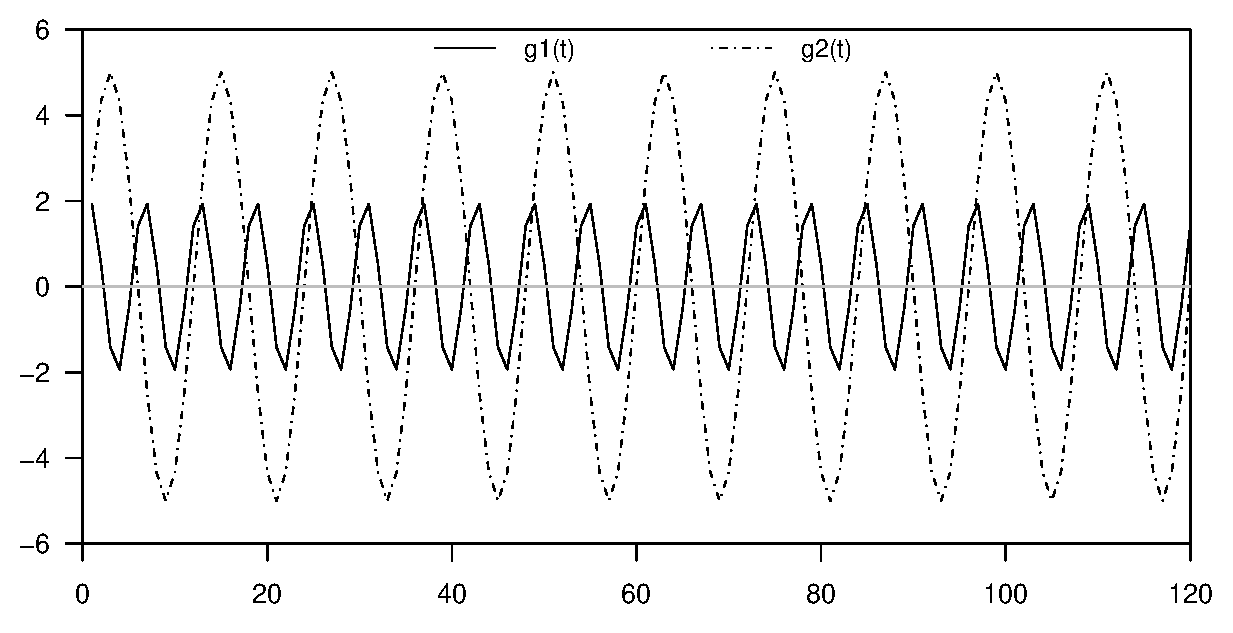
\includegraphics[width=.6\textwidth]
     {Chapter9Forecasting/TrigFctb.eps}
    \caption{\label{F9:TrigFctb} \small Plot of Two
Trigonometric Functions. Here, g$_1(t)$ has amplitude $a_1=5$ ,
frequency $f_1=2 \pi /12$ and phase shift $b_1=0$. Further, g$_2(t)$
has amplitude $a_2=2$, frequency $f_2=4 \pi/12 $ and phase shift
$b_2=\pi/4$.}
  \end{center}
\end{figure}


\bigskip

\begin{figure}[htp]
  \begin{center}
     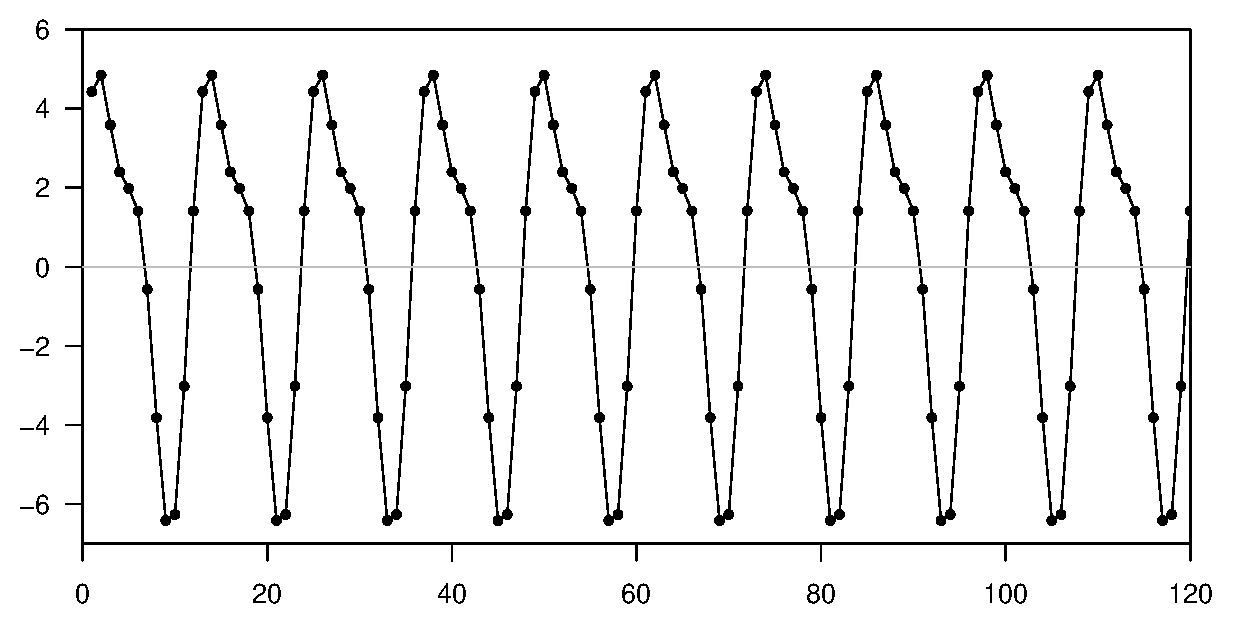
\includegraphics[width=.6\textwidth]
     {Chapter9Forecasting/TrigFctSum.eps}
    \caption{\label{F9:TrigFctSum} \small Plot of Sum of Two Trigonometric Functions in Figure \ref{F9:TrigFctb}.}
  \end{center}
\end{figure}


Consider the model $y_t=\beta_0+S_t+\varepsilon_t$, where $S_t$ is
specified in equation (\ref{E9:SeasonalEffect}). Because $\sin
(f_it)$ and $\cos (f_it)$ are functions of time, they can be treated
as known explanatory variables. Thus, the model
\begin{equation*}
y_t = \beta_0 + \sum_{i=1}^{m}\left\{ \beta_{1i}\sin (f_i t) +
\beta_{2i} \cos (f_i t)\right\} + \varepsilon_t
\end{equation*}
is a multiple linear regression model with $k=2m$ explanatory
variables. This model can be estimated using standard statistical
regression software. Further, we can use our variable selection
techniques to choose $m$, the number of trigonometric functions. We
note that $m$ is at most $SB/2$, for $SB$ even. Otherwise, we would
have perfect collinearity because of the periodicity of the sine
function. The following example demonstrates how to choose $m$.

\linejed

\empexjed{PrescriptionDrug}\index{datasets!prescription drugs}

\textbf{Example: Cost of Prescription Drugs.}\ecaptionjed{Cost of
Prescription Drugs} We consider a series from the State of New
Jersey's Prescription Drug Program, the cost per prescription claim.
This monthly series is available over the period August, 1986
through March, 1992, inclusive.

Figure \ref{F9:NJPrescTS} shows that the series is clearly
nonstationary, in that cost per prescription claims are increasing
over time. There are a variety of ways of handling this trend. One
may begin with a linear trend in time and include lag claims to
handle autocorrelations. For this series, a good approach to the
modeling turns out to be to consider the percentage changes in the
cost per claim series. Figure \ref{F9:NJPrescPChangeTS} is a time
series plot of the percent changes. In this figure, we see that many
of the trends that were evident in Figure \ref{F9:NJPrescTS} have
been filtered out.

\begin{figure}[htp]
  \begin{center}
     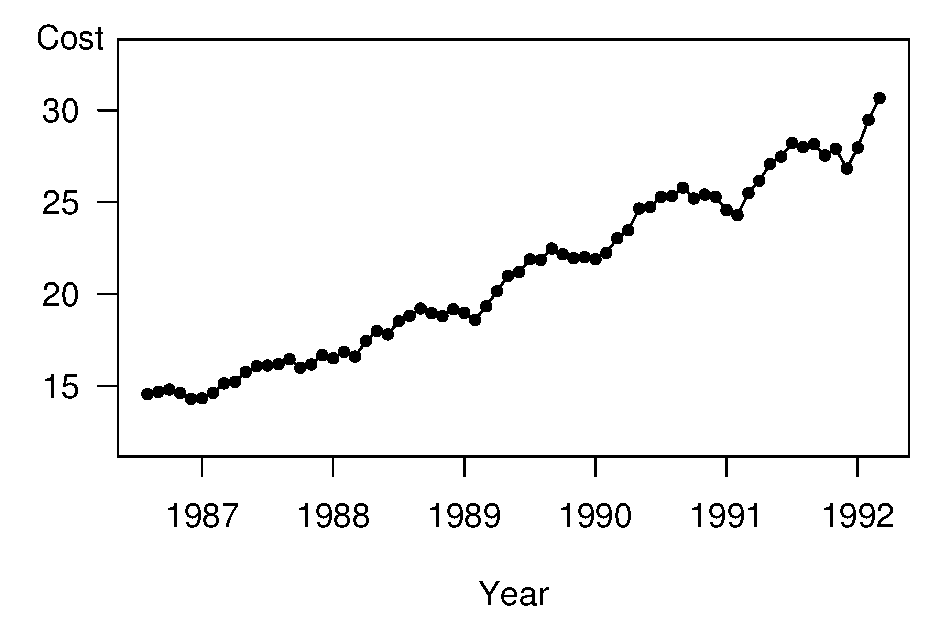
\includegraphics[width=.6\textwidth]
     {Chapter9Forecasting/NJPrescTS.eps}
    \caption{\label{F9:NJPrescTS} \small Time Series
Plot of Cost per Prescription Claim of the State of New Jersey's
Prescription Drug Plan.}
  \end{center}
\end{figure}

\bigskip

\begin{figure}[htp]
  \begin{center}
    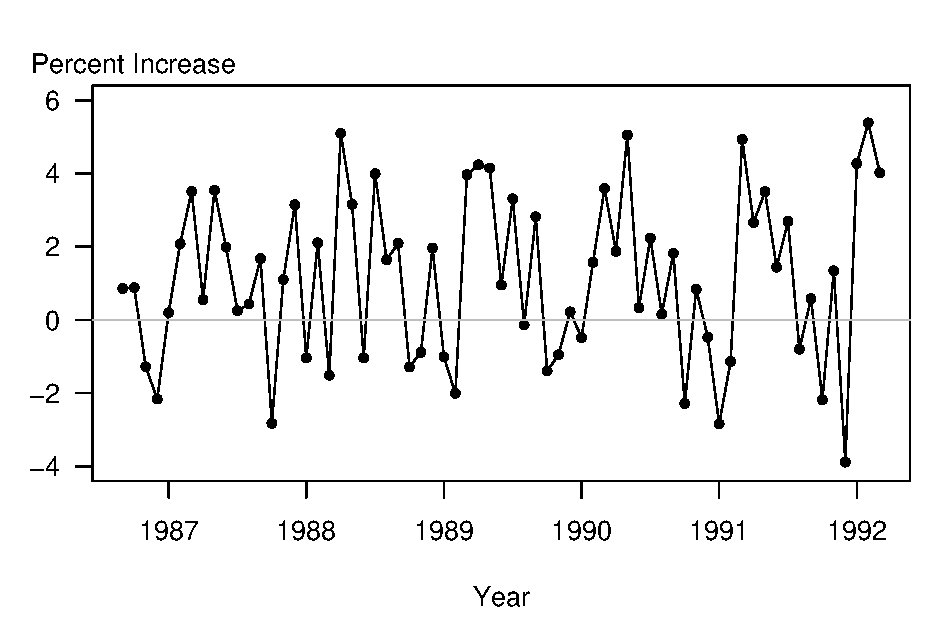
\includegraphics[width=.6\textwidth]
     {Chapter9Forecasting/NJPrescPChangeTS.eps}
    \caption{\label{F9:NJPrescPChangeTS} \small Monthly Percentage Changes of the Cost per Prescription
Claim.}
  \end{center}
\end{figure}


Figure \ref{F9:NJPrescPChangeTS} displays some mild seasonal
patterns in the data. A close inspection of the data reveals higher
percentage increases in the spring and lower increases in the fall
months. A trigonometric function using $m=1$ was fit to the data;
the fitted model is
\begin{center}
\begin{tabular}{cccc}
$\widehat{y}_t=$ & $1.2217$ & $-1.6956\sin (2\pi t/12)$ &
$+0.6536\cos
(2\pi t/12)$ \\
{\small std errors} & {\small (0.2325)} & {\small (0.3269)} &
{\small
(0.3298)} \\
{\small $t$-statistics} & {\small [5.25]} & {\small [-5.08]} &
{\small [1.98]}
\end{tabular}\end{center}

\noindent with $s=1.897$ and $R^2=31.5$ percent. This model reveals
some important seasonal patterns. The explanatory variables are
statistically significant and an $F$-test establishes the
significance of the model. Figure \ref{F9:NJPrescSeason} shows the
data with fitted values from the model superimposed. These
superimposed fitted values help to detect visually the seasonal
patterns.


\begin{figure}[htp]
  \begin{center}
    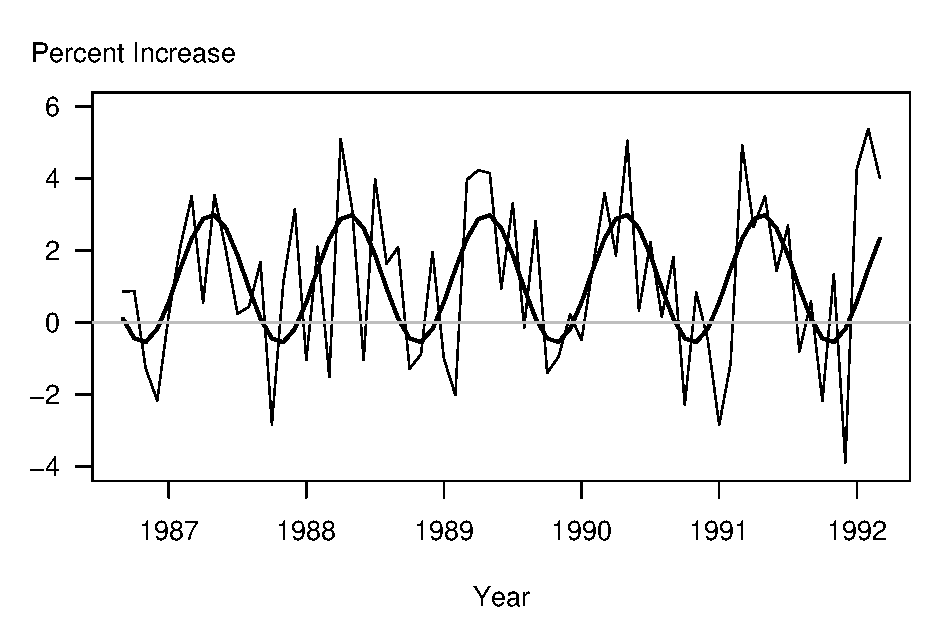
\includegraphics[width=.6\textwidth]
     {Chapter9Forecasting/NJPrescSeason.eps}
    \caption{\label{F9:NJPrescSeason} \small Monthly
Percentage Changes of the Cost per Prescription claim. Fitted values
from the seasonal trigonometric model have been superimposed.}
  \end{center}
\end{figure}


Examination of the residuals from this fitted model revealed few
further patterns. In addition, the model using $m=2$ was fit to the
data, resulting in $R^2 = 33.6$ percent. We can decide whether to
use $m=1$ or $2$ by considering the model
\begin{equation*}
y_t = \beta_0 + \sum_{i=1}^2 \left\{ \beta_{1i} \sin (f_i t) +
\beta_{2i} \cos (f_i t)\right\} + \varepsilon_t
\end{equation*}
and testing $H_0:\beta_{12} = \beta_{22}=0$. Using the partial
$F$-test, with $n=67, k=p=2$, we have
\begin{equation*}
F-ratio=\frac{(0.336-0.315)/2}{(1.000-0.336)/62} = 0.98.
\end{equation*}
With $df_1=p=2$ and $df_2=n-(k+p+1)=62$, the 95$th$ percentile of
the $F$-distribution is $F$-value = 3.15. Because $F-ratio<F-value$,
we can not reject $H_0$ and conclude that $m=1$ is the preferred
choice.

Finally, it is also of interest to see how our model of the
transformed data works with our original data, in units of cost per
prescription claim. Fitted values of percentage increases were
converted back to fitted values of cost per claim. Figure
\ref{F9:NJPrescFits} shows the original data with fitted values
superimposed. This figure establishes the strong relationship
between the actual and fitted series.


\begin{figure}[htp]
  \begin{center}
    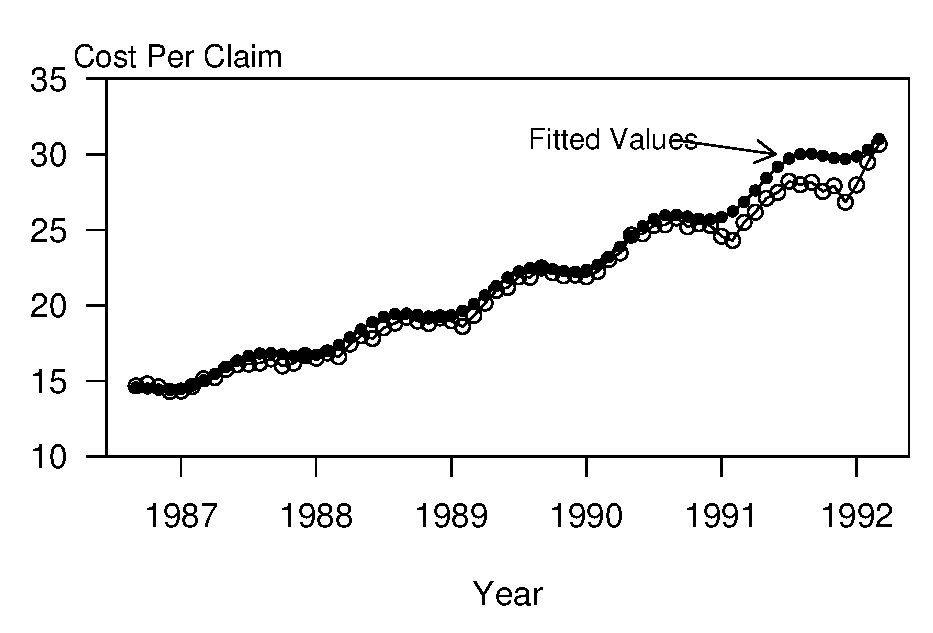
\includegraphics[width=.6\textwidth]
     {Chapter9Forecasting/NJPrescFits.eps}
    \caption{\label{F9:NJPrescFits} \small Monthly Percentage Changes of the Cost per Prescription
Claim. Fitted values from the seasonal trigonometric model have been
superimposed.}
  \end{center}
\end{figure}

\linejed

\subsubsection*{Seasonal Autoregressive Models}\index{time series models!seasonal autoregressive}

In Chapter 8 we examined patterns through time using
autocorrelations of the form $\rho_{k}$, the correlation between
$y_t$ and $y_{t-k}$. We constructed representations of these
temporal patterns using autoregressive models, regression models
with lagged responses as explanatory variables. Seasonal time
patterns can be handled similarly. We define the \emph{seasonal
autoregressive model of order P, SAR(P)}, as
\begin{equation}\label{E9:SAR(P)}
y_t=\beta_0+\beta_1y_{t-SB}+\beta_2y_{t-2SB}+\ldots+\beta
_{P}y_{t-PSB}+\varepsilon_t,
\end{equation}
where $SB$ is the seasonal base of under consideration. For example,
using $ SB=12$, a seasonal model of order one, $SAR(1)$, is
\begin{equation*}
y_t=\beta_0+\beta_1y_{t-12}+\varepsilon_t.
\end{equation*}
Unlike the $AR(12)$ model defined in Chapter 9, for the $SAR(1)$
model we have omitted $y_{t-1},y_{t-2},\ldots,y_{t-11}$ as
explanatory variables, although retaining $y_{t-12}$.

Just as in Chapter 8, choice of the order of the model is accomplished by
examining the autocorrelation structure and using an iterative model fitting
strategy. Similarly, the choice of seasonality $SB$ is based on an
examination of the data. We refer the interested reader to Abraham and
Ledolter (1983).

\linejed\index{datasets!prescription drugs}

\textbf{Example: Cost of Prescription Drugs - Continued.} Table
\ref{T9:PrescAutoCorr} presents autocorrelations for the percentage
increase in cost per claim of prescription drugs. There are $T=67$
observations for this data set, resulting in approximate standard
error of $se(r_{k})=1/\sqrt{67}\approx 0.122$. Thus,
autocorrelations at and around lags 6, 12, and 18 appear to be

\begin{table}[h]
\scalefont{0.9} \caption{\label{T9:PrescAutoCorr} Autocorrelations
of Cost per Prescription Claims}
\begin{center}
\begin{tabular}{c|ccccccccc}
\hline
$k$ & 1 & 2 & 3 & 4 & 5 & 6 & 7 & 8 & 9 \\
$r_{k}$ & 0.08 & 0.10 & -0.12 & -0.11 & -0.32 & -0.33 & -0.29 & 0.07 & 0.08
\\ \hline
$k$ & 10 & 11 & 12 & 13 & 14 & 15 & 16 & 17 & 18 \\
$r_{k}$ & 0.25 & 0.24 & 0.31 & -0.01 & 0.14 & -0.10 & -0.08 & -0.25 & -0.18
\\ \hline
\end{tabular}\end{center}
\scalefont{1.1111} \end{table}

\noindent significantly different than zero. This suggests using
$SB=6$. Further examination of the data suggested a $SAR(2)$ model.
The resulting fitted model is:

\begin{center}
\begin{tabular}{cccc}
$\widehat{y}_t=$ & $1.2191$ & $-0.2867y_{t-6}$ & $+0.3120y_{t-12}$ \\
{\small std errors} & {\small (0.4064)} & {\small (0.1502)} &
{\small
(0.1489)} \\
{\small t-statistics} & {\small [3.00]} & {\small [-1.91]} & {\small
[2.09]}
\end{tabular}
\end{center}

\noindent with $s=2.156$. This model was fit using conditional least
squares. Note that because we are using $y_{t-12}$ as an explanatory
variable, the first residual that can be estimated is 13. That is,
we lose twelve observations when lagging by twelve when using least
squares estimates.

\linejed

\subsubsection*{Seasonal Exponential Smoothing}\index{time series models!seasonal exponential smoothing}

An exponential smoothing method that has enjoyed considerable
popularity among forecasters is the Holt-Winter additive seasonal
model. Although it is difficult to express forecasts from this model
as a weighted least squares estimates, the model does appear to work
well in practice.

Holt (1957) introduced the following generalization of the double
exponential smoothing method. Let $w_1$ and $w_2$ be smoothing
parameters and calculate recursively the parameter estimates:

\begin{eqnarray*}
b_{0,t} &=&(1-w_1)y_t+w_1(b_{0,t-1}+b_{1,t-1}) \\
b_{1,t} &=&(1-w_2)(b_{0,t}-b_{0,t-1})+w_2b_{1,t-1} .
\end{eqnarray*}
These estimates can be used to forecast the linear trend model, $y_t
= \beta_0 + \beta_1 t + \varepsilon_t$. The forecasts are
$\widehat{y}_{T+l} = b_{0,T} + b_{1,T}~l$. With the choice
$w_1=w_2=2w/(1+w)$, the Holt procedure can be shown to produce the
same estimates as the double exponential smoothing estimates
described in Section \ref{S9:ExponSmooth}. Because there are two
smoothing parameters, the Holt procedure is a generalization of the
doubly exponentially smoothed procedure. With two parameters, we
need not use the same smoothing constants for the level ($\beta_0$)
and the trend ($\beta_1$) components. This extra flexibility has
found appeal with some data analysts.

Winters (1960) extended the Holt procedure to accommodate seasonal
trends. Specifically, the \emph{Holt-Winter seasonal additive model}
is
\begin{equation*}
y_t = \beta_0 + \beta_1 t + S_t + \varepsilon_t
\end{equation*}
where $S_t=S_{t-SB},S_1+S_2+\ldots+S_{SB}=0$, and $SB$ is the
seasonal base. We now employ three smoothing parameters: one for the
level, $w_1$, one for the trend, $w_2$, and one for the seasonality,
$w_{3}$. The parameter estimates for this model are determined
recursively using:
\begin{eqnarray*}
b_{0,t} &=&(1-w_1)\left( y_t-\widehat{S}_{t-SB}\right)
+w_1(b_{0,t-1}+b_{1,t-1}) \\
b_{1,t} &=&(1-w_2)(b_{0,t}-b_{0,t-1})+w_2b_{1,t-1} \\
\widehat{S}_t &=&(1-w_{3})\left( y_t-b_{0,t}\right)
+w_{3}\widehat{S} _{t-SB}.
\end{eqnarray*}
With these parameter estimates, forecasts are determined using:
\begin{equation*}
\widehat{y}_{T+l}=b_{0,T}+b_{1,T}~l+\widehat{S}_T(l)
\end{equation*}
where $\widehat{S}_T(l)=\widehat{S}_{T+l}$ for $l=1,2,\ldots,SB$,
$\widehat{S} _T(l)=\widehat{S}_{T+l-SB}$ for $l=SB+1,\ldots,2SB$,
and so on.

In order to compute the recursive estimates, we must decide on (i)
initial starting values and (ii) a choice of smoothing parameters.
To determine initial starting values, we recommend fitting a
regression equation to the first portion of the data. The regression
equation will include a linear trend in time, $\beta_0 + \beta_1 t$,
and $SB-1$ binary variables for seasonal variation. Thus, only
$SB+1$ observations are required to determine initial estimates
$b_{0,0}, b_{1,0}, y_{1-SB}, y_{2-SB},\ldots, y_0$.

Choosing the three smoothing parameters is more difficult. Analysts
have found it difficult to choose three parameters using an
objective criterion, such as the minimization of the sum of squared
one-step prediction errors, as in Section \ref{S9:ExponSmooth}. Part
of the difficulty stems from the nonlinearity of the minimization,
resulting in prohibitive computational time. Another part of the
difficulty is that functions such as the sum of squared one-step
prediction errors often turn out to be relatively insensitive to the
choice of parameters. Analysts have instead relied on rules of thumb
to guide the choice of smoothing parameters. In particular, because
seasonal effects may take several years to develop, a lower value of
$w_{3}$ is recommended (resulting in more smoothing). Cryer and
Miller (1994) recommend $w_1=w_2=0.9$ and $w_{3}=0.6$.

\section{Unit Root Tests}\index{time series terms and
concepts!unit root tests}

We have now seen two competing models that handle nonstationary with
a mean trend, the linear trend in time model and the random walk
model. Section 7.6 illustrated how we can choose between these two
models on a out-of-sample basis. For a selection procedure based on
in-sample data, consider the model
\begin{equation*}
y_t = \mu_0 +  \phi (y_{t-1} - \mu_0) + \mu_1 \left(  \phi +
(1-\phi) t \right) + \varepsilon_t.
\end{equation*}
When $\phi =1$, this reduces to a random walk model with $y_t=\mu
_1+y_{t-1}+\varepsilon_t.$\ When $\phi <1$ and $\mu_1=0$, this
reduces to an $AR(1)$ model, $y_t=\beta_0+\phi y_{t-1}+\varepsilon
_t, $ with $\beta_0=\mu_0\left( 1-\phi \right) .$ When $\phi =0$,
this reduces to a linear trend in time model with $y_t = \mu_0 +
\mu_1 t + \varepsilon_t.$

Running a model where the left-hand side variable is potentially a
random walk is problematic. Hence, it is customary to use least
squares on the model
\begin{equation}\label{E9:DickeyFuller1}
y_t-y_{t-1}=\beta_0+\left( \phi -1\right) y_{t-1}+\beta
_1t+\varepsilon_t
\end{equation}
where we interpret $\beta_0=\mu_0\left( 1-\phi \right) + \phi \mu_1$
and $\beta_1=\mu_1\left( 1-\phi \right).$ From this regression, let
$ t_{DF}$ be the $t$-statistic associated with the $y_{t-1}$
variable. We wish to use the $t$-statistic to test the null
hypothesis that $H_0:\phi =1$ versus the one-sided alternative that
$H_{a}:\phi <1$. Because $\{y_{t-1}\}$ is a random walk process
under the null hypothesis, the distribution of $ t_{DF}$\ does not
follow the usual $t$-distribution but rather follows a special
distribution, due to Dickey and Fuller (1979). This distribution has
been tabulated has been programmed in several statistical packages,
Fuller (1996).\index{time series statistics!Dickey-Fuller}

\linejed\index{datasets!labor force participation rates}

\textbf{Example: Labor Force Participation Rates -
Continued.}\ecaptionjed{Labor Force Participation Rates} We
illustrate the performance of the Dickey-Fuller tests on the labor
force participation rates introduced in Chapter 7. There, we
established that the series was clearly non-stationary and that
out-of-sample forecasting showed the random walk to be preferred
when compared to the linear trend in time model.

Table \ref{T9:DFStats} summarizes the test. Both without ($\mu_1 =
0$) and with ($\mu_1 \neq 0$) the trend line, the $t$-statistic
($t_{DF}$) is statistically insignificant (compared to the 10\%
critical value). This provides evidence that the random walk is the
preferred model choice.

\begin{table}[h]
\scalefont{0.9} \caption{\label{T9:DFStats} Dickey-Fuller Test
Statistics with Critical Values}
\begin{center}
\begin{tabular}{c|cccc}
\hline
& \multicolumn{2}{|c}{Without Trend} & \multicolumn{2}{c}{With Trend} \\
\cline{2-5}
&  & 10\% Critical  &  & 10\% Critical  \\
Lag ($p$)& $t_{DF}$ & Value & $t_{DF}$ & Value \\ \hline
& -1.614 & -2.624 & -0.266 & -3.228 \\
1 & -1.816 & -2.625 & -0.037 & -3.230 \\
2 & -1.736 & -2.626 &  0.421 & -3.233 \\ \hline
\end{tabular}\end{center}
\scalefont{1.1111} \end{table}

\linejed
\bigskip

One criticism of the Dickey-Fuller test is that the disturbance term
in equation (\ref{E9:DickeyFuller1}) is presumed to be serially
uncorrelated. To protect against this, a commonly used alternative
is the \emph{augmented Dickey-Fuller} test statistic. This is the
$t$-statistic associated with the $y_{t-1}$ variable using ordinary
least squares on the following equation
\begin{equation}\label{E9:DickeyFuller2}
y_t-y_{t-1}=\beta_0+\left( \phi -1\right) y_{t-1}+\beta
_1t+\sum_{j=1}^{p}\phi_{j}\left( y_{t-j}-y_{t-j-1}\right)
+\varepsilon_t.
\end{equation}\index{time series statistics!augmented Dickey-Fuller}
In this equation, we have augmented the disturbance term by
autoregressive terms in the differences \{$y_{t-j}-y_{t-j-1}$\}.\
The idea is that these terms serve to capture serial correlation in
the disturbance term. Research has not reached consensus on how to
choose the number of lags ($p$) - in most applications, analysts
provide results of the test statistic for a number of choices of
lags and hope that conclusions reached are qualitatively similar.
This is certainly the case for the labor force participation rates
as demonstrated in Table \ref{T9:DFStats}. Here, we see that for
each lag choice, the random walk null hypothesis can not be
rejected.

\section{ARCH/GARCH Models}

To this point, we have focussed on forecasting the level of the
series - \ that is, the conditional mean. However, there are
important applications, notably in the study of finance, where
forecasting the variability is important. To illustrate, the
variance plays a key role in option pricing, such as when using the
Black-Scholes formula.

Many financial time series exhibit \emph{volatility clustering},
that is, periods of high volatility (large changes in the series)
followed by periods of low volatility. To illustrate, consider the
following.

\linejed

\empexjed{SP500Daily}\index{datasets!Standard and Poor's daily
returns}

\textbf{Example: S \& P 500 Daily Returns.}\ecaptionjed{S \& P 500
Daily Returns} Figure \ref{F9:SandPDailyTS}  provides a time series
plot of daily returns from the Standard \& Poor's 500 over the
period 2000-2006, inclusive. Here, we see the early part of the
series, prior to January of 2003 is more volatile when compared to
the latter part of the series. Except for the changing volatility,
the series appears to be stationary, without dramatic increases or
decreases.

\begin{figure}[htp]
  \begin{center}
    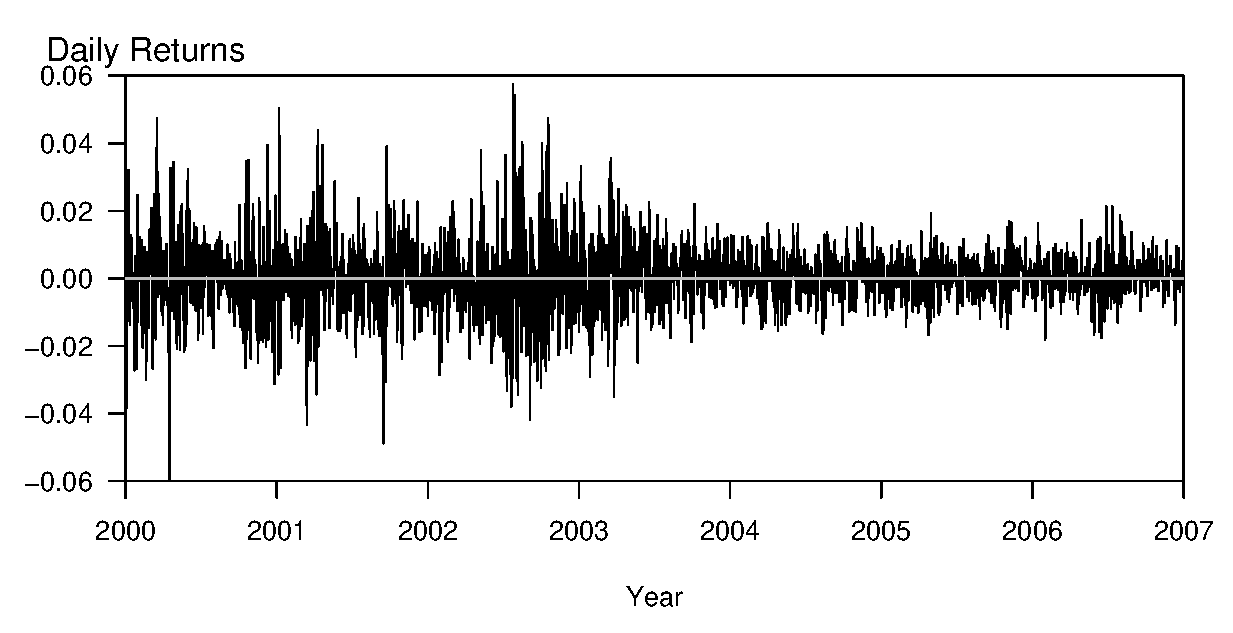
\includegraphics[width=.8\textwidth]
     {Chapter9Forecasting/SandPDailyTS.eps}
    \caption{\label{F9:SandPDailyTS} \small Time Series Plot of Daily S\&P Returns, 2000-2006, inclusive.}
  \end{center}
\end{figure}

\linejed

The concept of variability changing over time seems at odds with our
notions of stationarity. This is because a condition for weak
stationary is that the series has a constant variance. The
surprising thing is that we can allow for changing variances by
conditioning on the past and still retain a weakly stationary model.
To see this mathematically, we use the notation $\Omega_t$ to denote
the information set, the collection of knowledge about the process
up to and including time $t$. For a weakly stationary series, we may
denote this as $\Omega
_t=\{\varepsilon_t,\varepsilon_{t-1},\ldots\}$. We allow the
variance to depend on time $t$ by conditioning on the past,
\begin{equation*}
\sigma_t^2=\mathrm{Var}_{t-1}\left( \varepsilon_t\right) =\mathrm{E}
\left( \left[ \varepsilon_t-\mathrm{E}\left( \varepsilon_t|\Omega
_{t-1}\right) \right] ^2|\Omega_{t-1}\right) .
\end{equation*}
We now present several parametric models of $\sigma_t^2$\ that
allows us to quantify and forecast this changing volatility.

\subsubsection*{ARCH Model}\index{time series models!autoregressive changing heteroscedasticity model of order
$p$, $ARCH(p)$}

The \emph{autoregressive changing heteroscedasticity model of order
p,} $ ARCH(p),$ is due to Engle (1982). We now assume that the
distribution of $ \varepsilon_t$\ given $\Omega_{t-1}$ is normally
distributed with mean zero and variance $\sigma_t^2$. We further
assume that the conditional variance is determined recursively by
\begin{equation*}
\sigma_t^2=w+\gamma_1\varepsilon_{t-1}^2+\ldots+\gamma
_{p}\varepsilon_{t-p}^2=w+\gamma (B)\varepsilon_t^2,
\end{equation*}
where $\gamma (x)=\gamma_1x+\ldots+\gamma_{p}x^{p}.$ Here, $w>0$\ is
the ``long-run'' volatility parameter and $
\gamma_1,\ldots,\gamma_p$\ are coefficients such that $\gamma _j
\geq 0$ and $\gamma (1)=\sum_{j=1}^{p} \gamma_j < 1$.

In the case that $p=1$, we can see that a large change to the series
$ \varepsilon_{t-1}^2$\ can induce a large conditional variance
$\sigma_t^2$. Higher orders of $p$ help capture longer term effects.
Thus, this model is intuitively appealing to analysts.
Interestingly, Engle provided additional mild conditions to assure
that the $\{\varepsilon_t\}$ is weakly stationarity. Thus, despite
having a changing \emph{conditional} variance, the
\emph{unconditional} variance remains constant over time.

\subsubsection*{GARCH Model}\index{time series models!generalized $ARCH$ model of order
$p$, $GARCH(p)$}

The \emph{generalized ARCH model of order p,} $GARCH(p,q),$
complements the $ ARCH$ model in the same way that the moving
average complements the autoregressive model. As with the $ARCH$
model, we assume that the distribution of $\varepsilon_t$\ given
$\Omega_{t-1}$ is normally distributed with mean zero and variance
$\sigma_t^2$. The conditional variance is determined recursively by
\begin{equation*}
\sigma_t^2-\delta_1\sigma_{t-1}^2+-\ldots-\delta_{q}\sigma
_{t-q}^2=w+\gamma_1\varepsilon_{t-1}^2+\ldots+\gamma_{p}\varepsilon
_{t-p}^2,
\end{equation*}
or $\sigma_t^2=w+\gamma (B)\varepsilon_t^2+\delta (B)\sigma_t^2,$
where $\delta (x)=\delta_1x+\ldots+\delta_{q}x^{q}.$ In addition to
the $ARCH(p)$ requirements, we also need $\delta_{j}\geq 0$ and
$\gamma (1)+\delta \left( 1\right) <1$.

As it turns out, the $GARCH(p,q)$\ is also a weakly stationary
model, with mean zero and (unconditional) variance
$\mathrm{Var~}\varepsilon_t=w/(1-\gamma (1)-\delta \left( 1\right)
).$

\linejed\index{datasets!Standard and Poor's daily returns}

\textbf{Example: S \& P 500 Daily Returns - Continued. }After an
examination of the data (details not given here), an $MA(2$) model
was fit to the series with $GARCH(1,1)$ errors. Specifically, if
$y_t$ denotes the daily return from the S \& P series, for
$t=1,\ldots,1759$, we fit the model
\begin{equation*}
y_t = \beta_0 + \varepsilon_t - \theta_1 \varepsilon_{t-1} -
\theta_2 \varepsilon_{t-2},
\end{equation*}
where the conditional variance is determined recursively by
\begin{equation*}
\sigma_t^2 - \delta_1 \sigma_{t-1}^2 = w + \gamma_1
\varepsilon_{t-1}^2.
\end{equation*}

The fitted model appears in Table \ref{T9:SandPDaily}. Here, the
statistical package we used employs maximum likelihood to determine
the estimated parameters as well as the standard errors needed for
the $t$-statistics. The $t$-statistics show that all parameter
estimates, except $\theta_1$, are statistically significant. As
discussed in Chapter 8, the convention is to retain lower order
coefficients, such as $\theta_1$, if higher order coefficients like
$\theta_2$ are significant. Note from Table \ref{T9:SandPDaily} that
the sum of the $ARCH$ coefficient ($\delta_1$) and the $GARCH$
coefficient ($\gamma_1$) are nearly one with $GARCH$ coefficient
substantially larger than the $ARCH$ coefficient. This phenomenon is
also reported by Diebold (2004, page 400) who states that it is
commonly found in studies of financial asset returns.

\bigskip


\begin{table}[h]
\scalefont{0.9} \caption{\label{T9:SandPDaily} S \& P 500 Daily
Returns Model Fit}
\begin{center}
\begin{tabular}{crr}
\hline Parameter & Estimate & $t$-statistic \\ \hline
$\beta_0$ & $0.0004616$ & $2.51$ \\
$\theta_1$ & $-0.0391526$ & $-1.49$ \\
$\theta_2$ & $-0.0612666$ & $-2.51$ \\
$\delta_1$ & $0.0667424$ & $6.97$ \\
$\gamma_1$ & $0.9288311$ & $93.55$ \\
$w$ & $5.61\times 10^{-7}$ & $2.30$ \\
Log-likelihood & $5,658.852$ &  \\ \hline
\end{tabular}\end{center}
\scalefont{1.1111} \end{table}

\linejed

\bigskip

\section{Further Reading and References}

For other variations of the running average method and exponential
smoothing, see Abraham and Ledolter (1983).


For a more detailed treatment of unit root tests, we refer the
reader to Diebold (2004) or Fuller (1996) for a more advanced
treatment.

\bigskip

\textbf{Chapter References}

\begin{multicols}{2}

\scalefont{0.9}

Abraham, Bovas and Ledolter, Johannes (1983). \textit{Statistical
Methods for Forecasting}. John Wiley \& Sons, New York.

Cryer, Jon D. and Robert B. Miller (1994). \textit{Statistics for
Business: Data Analysis and Modelling}. PWS-Kent, Boston.

Dickey, D. A. and Wayne A. Fuller (1979). Distribution of the
estimators for autoregressive time series with a unit root.
\textit{Journal of the American Statistical Association} 74,
427-431.

Diebold, Francis X. (2004). \textit{Elements of Forecasting}, Third Edition.
Thomson, South-Western, Mason Ohio.

Engle, R. F. (1982). Autoregressive conditional heteroscedasticity
with estimates of UK inflation. \textit{Econometrica} 50, 987-1007.

Fuller, Wayne A. (1996). \textit{Introduction to Statistical Time
Series, Second Edition.} John Wiley \& Sons, New York.

Holt, C. C. (1957). Forecasting trends and seasonals by
exponenetially weighted moving averages. \textit{O.N.R. Memorandum},
No. 52, Carnegie Institute of Technology.

Winters, P. R. (1960). Forecasting sales by exponentially weighted
moving averages. \textit{Management Science} 6, 324-342.

\scalefont{1.1111}

\end{multicols}
